This chapter describes the methodology used to generate counterfactual explanations using Variational Autoencoders (VAEs) and evaluate different feature masking strategies to enhance interpretability in autonomous driving systems. The methodology consists of multiple stages, including dataset collection, VAE training, classifier training, feature masking, counterfactual explanation generation.

A high-level workflow of the methodology is shown in Figure (let im edraw the methodology diagram and place an image). The dataset is collected from the CARLA simulator, preprocessed, and used to train a Variational Autoencoder (VAE) for latent space representation. A classifier is trained to distinguish between "STOP", "GO", "RIGHT, and "LEFT" decisions based on input images. Counterfactual explanations are generated by applying different feature masking techniques to alter the image or latent space representation. Finally, the counterfactuals are evaluated using both AI-based quantitative metrics and human evaluation studies.

\section{Experimental Setup}

All experiments in this thesis were conducted in a Linux environment to ensure compatibility with the CARLA simulator and associated tools. The setup was built using \textbf{CARLA version 0.9.15}, an open-source urban driving simulator widely adopted for autonomous driving research. This version provides a flexible and high-fidelity simulation environment, making it suitable for collecting diverse, labeled driving data under various rural and urban conditions.

To maintain compatibility with CARLA’s Python API, \textbf{Python version 3.7} was used for dataset collection. This version is recommended by CARLA’s developers to avoid API and dependency conflicts. The dataset was collected using two CARLA maps \textbf{Town03} and \textbf{Town07} \cite{CARLA2024}, provide varied driving topologies as shown in Figure~\ref{fig:carla_maps}. These maps were chosen due to their varied road layouts and environmental features, which provide rich scenarios for evaluating counterfactual explanations. Example simulation scenes demonstrating diverse driving and weather conditions are presented in Figure~\ref{fig:carla_scenes}. Users replicating this setup should download the CARLA server (v0.9.15) along with the additional maps from the \textit{official CARLA repository}. Once downloaded, the maps must be copied into the main CARLA directory to ensure proper integration.

\begin{figure}[htbp]
    \centering
    \begin{subfigure}{0.48\textwidth}
        \centering
        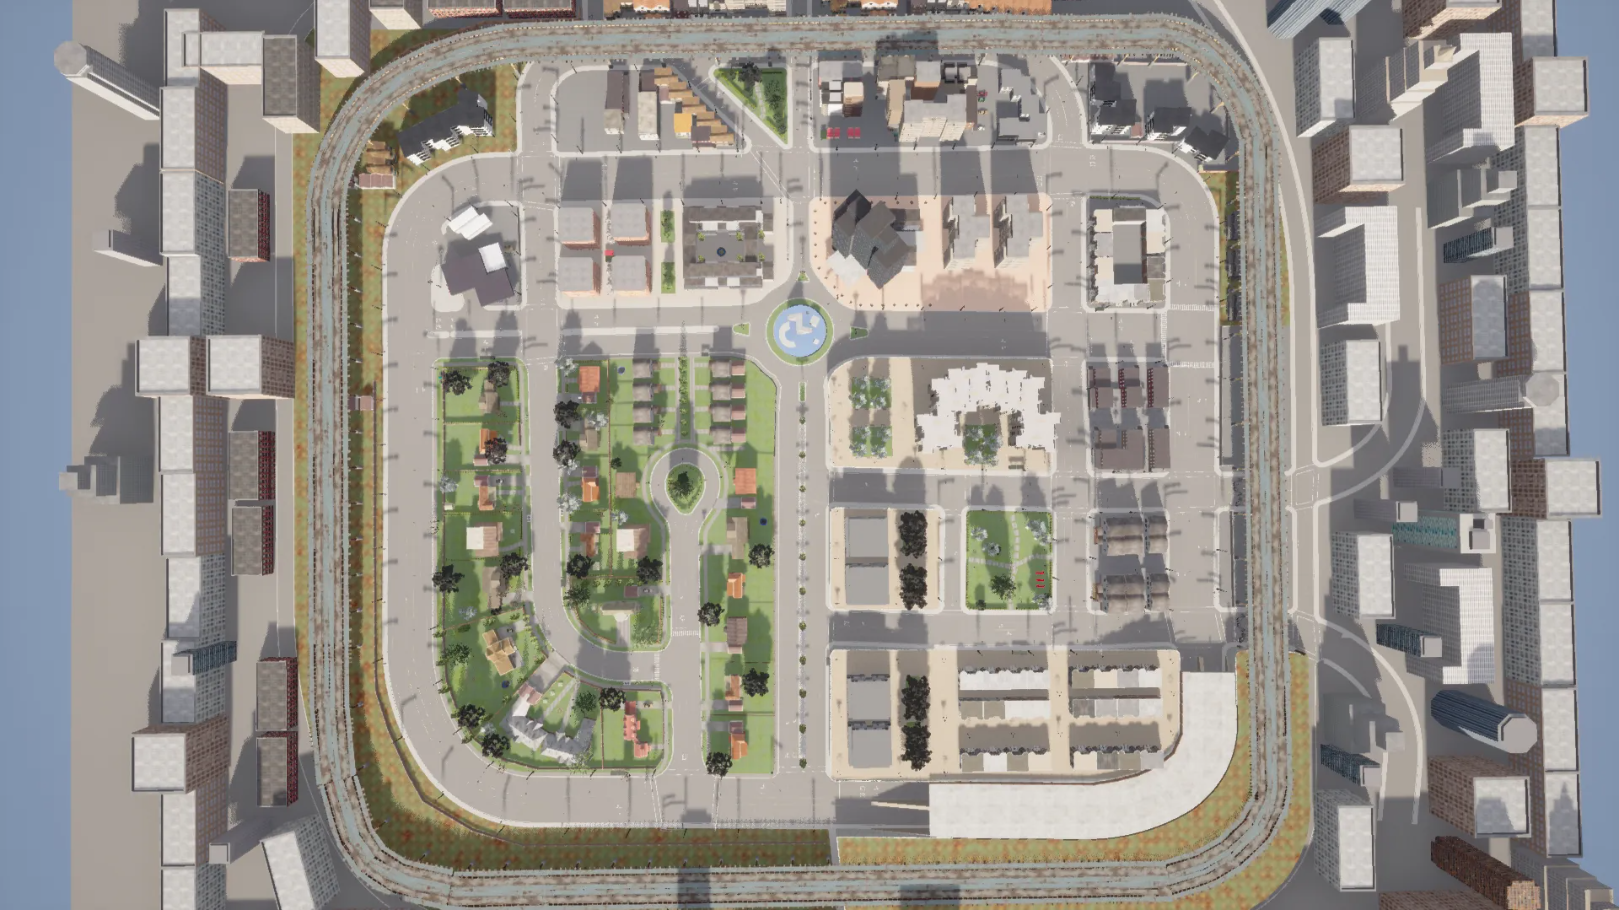
\includegraphics[width=\linewidth]{img/carla/town03.png}
        \caption{CARLA Town03 layout}
    \end{subfigure}
    \hfill
    \begin{subfigure}{0.48\textwidth}
        \centering
        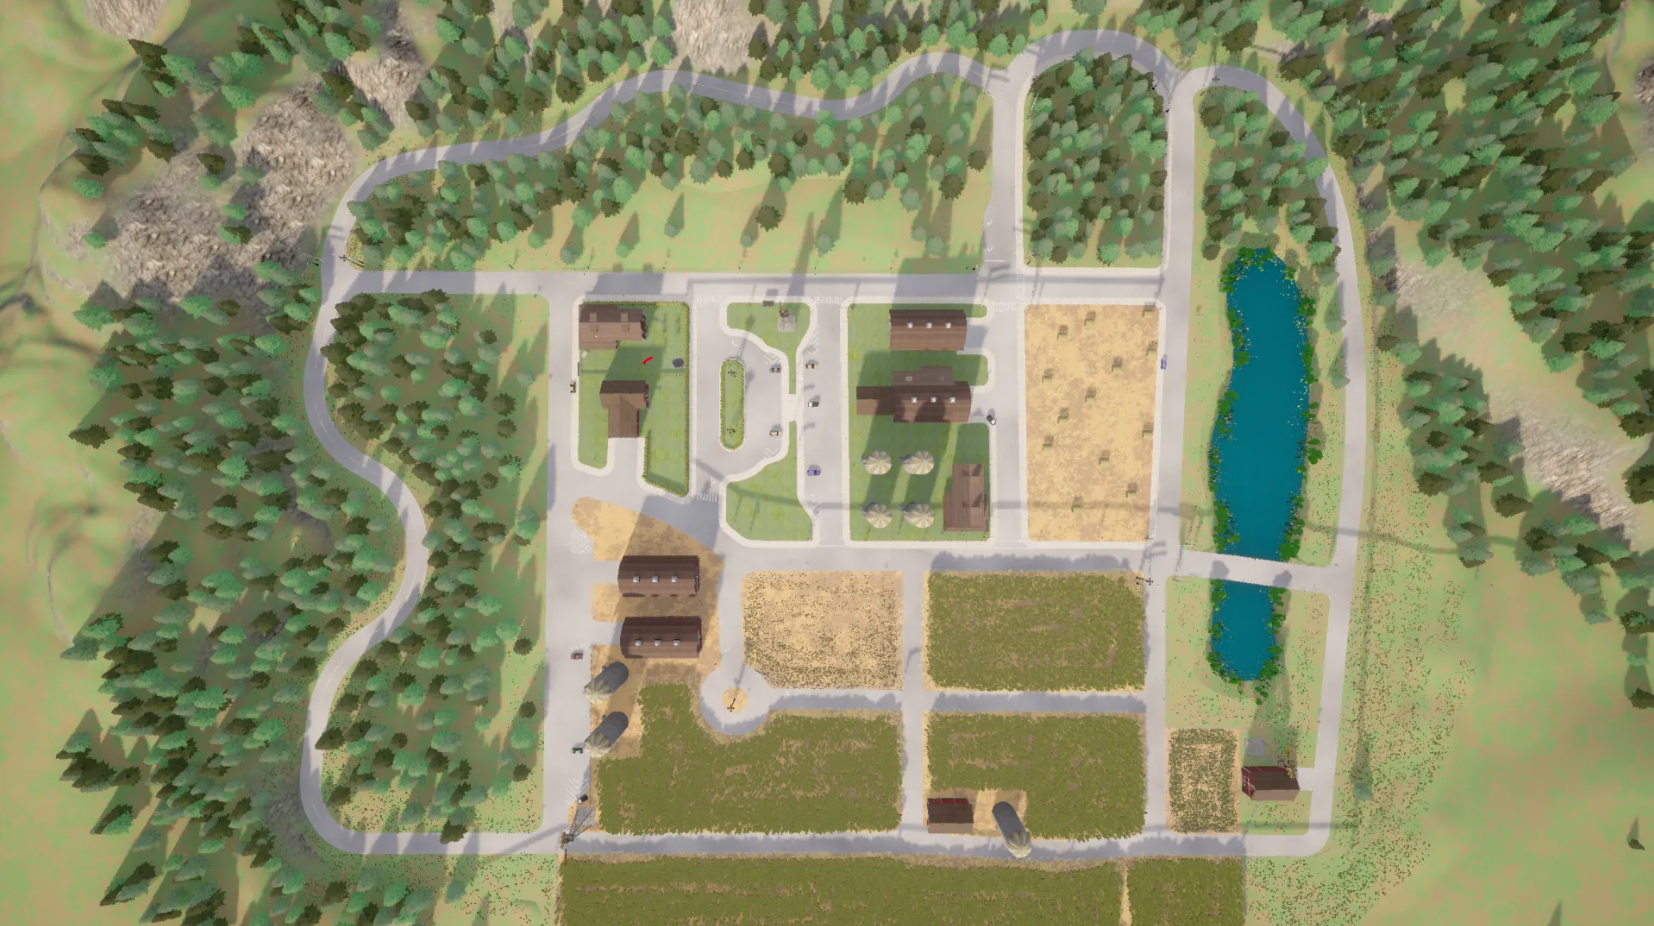
\includegraphics[width=\linewidth]{img/carla/town_7.png}
        \caption{CARLA Town07 layout}
    \end{subfigure}
    \caption{Top-down map layouts of the selected CARLA towns used for dataset collection~\cite{CARLA2024}}.
    \label{fig:carla_maps}
\end{figure}

\begin{figure}
    \centering
    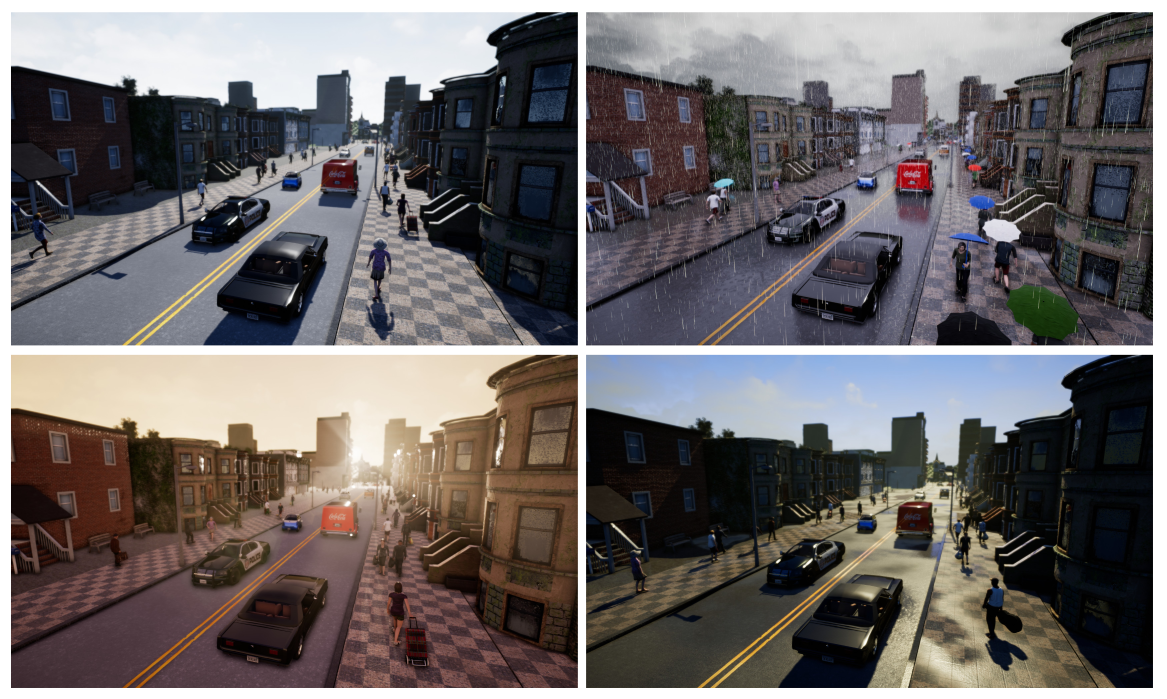
\includegraphics[width=0.7\linewidth]{img/carla/CARLA_Environment.png}
    \caption{3D Sample scenes from CARLA showcasing diverse conditions during dataset collection. The images illustrate a variety of urban and rural settings, with diverse lighting and weather conditions, including sunny, foggy, rainy, and snowy scenarios. Each scene highlights the flexibility of CARLA in simulating realistic driving environments for autonomous vehicle testing.}
    \label{fig:carla_scenes}
\end{figure}


Before executing any client-side scripts for dataset collection, it is essential to start the CARLA server using the following command in the CARLA root directory: ./CarlaUE4.sh


This launches the CARLA simulation in the Unreal Engine environment. For smooth operation, it is recommended to run the project on a system with at least \textbf{16 GB of RAM}, a dedicated GPU (e.g., \textbf{NVIDIA RTX series}), and \textbf{Ubuntu 18.04 or 20.04 LTS}. 

For the development and training of the Variational Autoencoder (VAE) and classifier models, we used \textbf{Python version 3.11 or higher}. This was necessary to avoid compatibility issues with newer versions of PyTorch, which are not well supported on older Python versions like 3.7. While dataset collection was handled using Python 3.7, the core machine learning model development required a more modern Python environment.  

To monitor and interpret various aspects of model training such as loss, accuracy, weight distributions, and layer activations we used \textbf{TensorBoard}. It provided valuable insights into training behavior and helped fine-tune model performance.

\section{Dataset Collection, Labeling, and Splitting Process}

To train and evaluate the proposed models effectively, a high-quality and well-structured dataset was essential. A systematic data preparation pipeline consisting of three key stages \textit{collection}, \textit{labeling}, and \textit{splitting}. The dataset was first collected using the CARLA simulator, which offers a controllable and realistic environment for simulating diverse driving scenarios. Following data collection, a precise rule-based labeling strategy was applied using vehicle control signals to assign meaningful class labels. Finally, the labeled dataset was partitioned into training and testing subsets to ensure class balance and prevent data leakage. This structured pipeline ensured consistency, and reproducibility  throughout the experimental workflow.

\subsection{Dataset Collection}

The dataset was collected using the CARLA simulator~\cite{CARLA2024docs}. An Audi A2 vehicle was deployed in autopilot mode to autonomously navigate the environment while capturing RGB images and corresponding control signals. A front mounted RGB camera was configured with a 125° field of view (FoV) and a resolution of $160 \times 80$ pixels. This resolution was selected to balance computational efficiency with sufficient visual detail for model learning.

A total of approximately 12,000 images were collected under varied driving scenarios. Each image was paired with the vehicle’s control parameters steering, throttle, and brake. The \textit{steering angle} ranged from $-1$ (full left) to $1$ (full right), while \textit{throttle} and \textit{brake} values ranged from $0$ to $1$, representing the intensity of acceleration and braking, respectively. This multi-modal data captured both visual context and driving behavior. The resulting dataset served as the foundation for both binary (STOP vs. GO) and multi-class (STOP, GO, LEFT, RIGHT) classification tasks.


\subsection{Dataset Labeling}

The collected data was labeled using a deterministic rule-based strategy derived from the vehicle’s control inputs. Two distinct labeling schemes were implemented to support binary and multi-class classification objectives.

For the \textbf{binary-class scheme}, each frame was labeled as either \texttt{STOP} or \texttt{GO}. A frame was labeled as \texttt{STOP} if the brake value exceeded a predefined threshold. Otherwise, it was labeled as \texttt{GO}. This distinction effectively captured the vehicle's motion state based on braking behavior.

For the \textbf{multi-class scheme}, labels were assigned based on prioritized control logic:
\begin{itemize}
    \item STOP, if the brake value exceeded a defined threshold.
    \item RIGHT, if the steering value was significantly positive and throttle was active.
    \item LEFT, if the steering value was significantly negative and throttle was active.
    \item GO, for all remaining cases where the vehicle moved straight without braking or significant steering.
\end{itemize}

This approach ensured mutually exclusive and semantically meaningful labels for each image. Threshold values for labeling were empirically determined based on the distribution of control signals across the dataset. The process was fully automated, ensuring reproducibility and eliminating manual labeling bias.

\subsection{Dataset Splitting}

Following labeling, the dataset was divided into separate training and testing subsets. The splitting was performed \textit{after} labeling to maintain label integrity and avoid any form of data leakage. Care was taken to ensure that the distribution of class labels remained balanced across both sets. This was critical for promoting fair learning and evaluation, particularly in the multi-class scenario.

The labeled dataset was partitioned using an 80/20 split ratio, where 80\% of the data was used for training and 20\% for testing. This ensured sufficient data for model learning while preserving a representative set for evaluation.

For the binary classification scheme, the training set contained 4,959 GO and 4,728 STOP samples, while the test set included 1,262 GO and 1,160 STOP samples, maintaining a near-balanced distribution across classes. Similarly, for the 4-class setting, all classes (GO, STOP, LEFT, RIGHT) were equally represented with 3,327 samples in training and 821 samples per class in testing. The distributions for both schemes are visualized side by side in Figure~\ref{fig:label_distribution_combined}.


\begin{figure}[htbp]
    \centering
    \begin{subfigure}{0.48\textwidth}
        \centering
        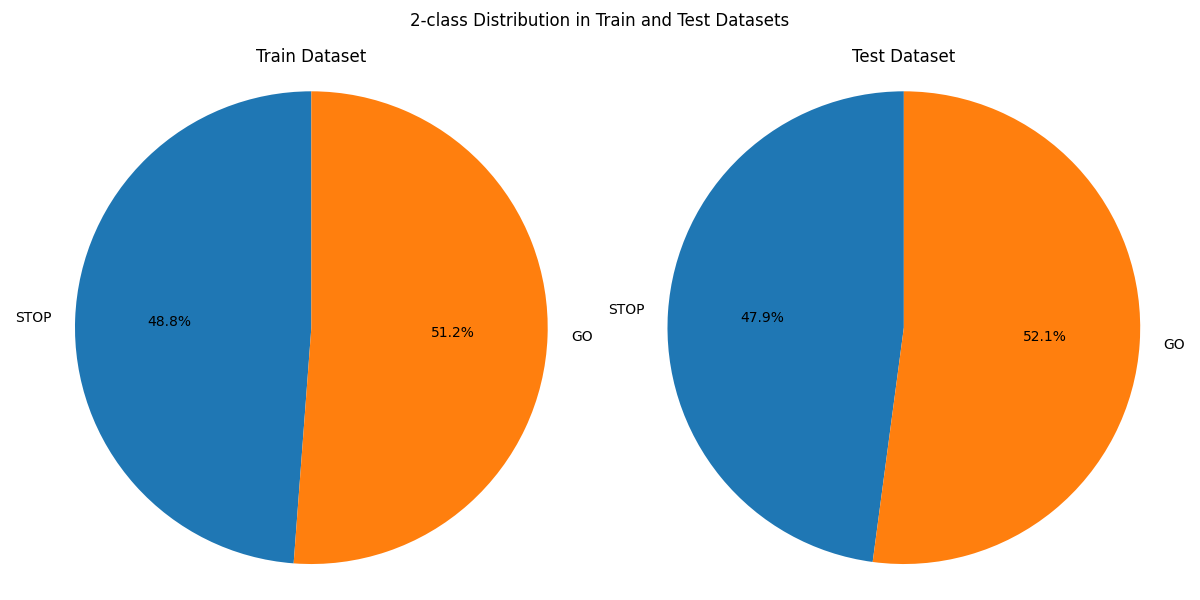
\includegraphics[width=\linewidth]{img/dataset/2class_distribution.png}
        \caption{Binary (GO/STOP) label distribution\vphantom{g}}
        \label{fig:binary_class_distribution}
    \end{subfigure}
    \hfill
    \begin{subfigure}{0.5\textwidth}
        \centering
        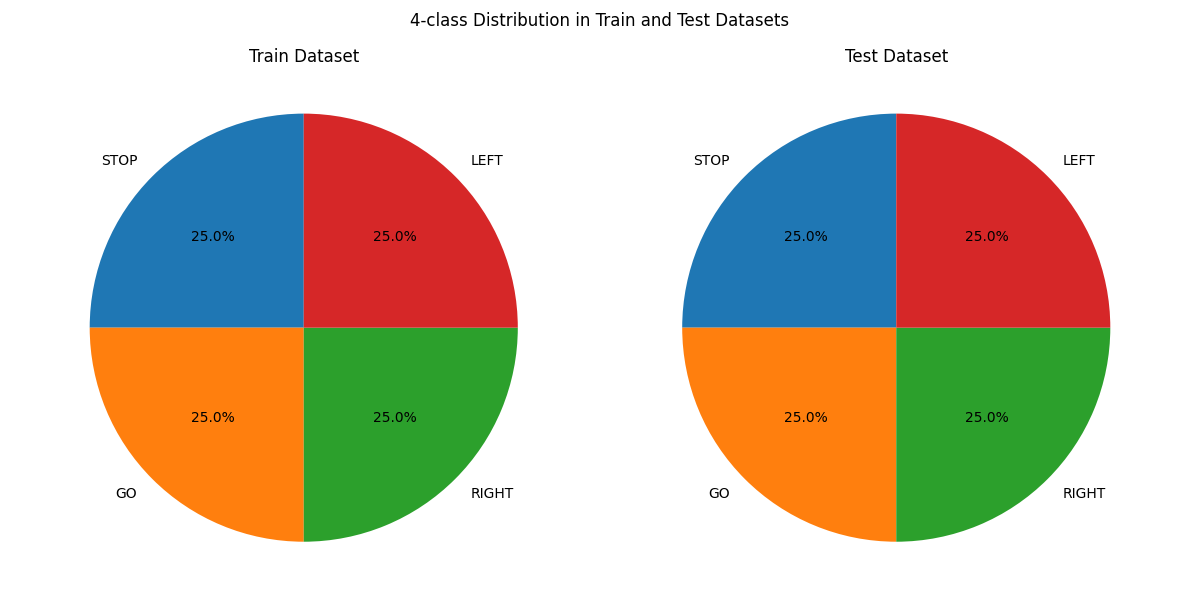
\includegraphics[width=\linewidth]{img/dataset/4class_distribution.png}
        \caption{4-class label distribution (GO, STOP, LEFT, RIGHT)}
        \label{fig:class_distribution_pie}
    \end{subfigure}
    \caption{Label distributions across training and testing datasets for binary and multi-class classification schemes.}
    \label{fig:label_distribution_combined}
\end{figure}





\section{Variational Autoencoder (VAE)} \label{sec:vae}

This section outlines the architectural design, training process, and evaluation protocol for the Variational Autoencoder (VAE) used in this work. The VAE serves as a generative backbone for producing realistic and plausible counterfactual explanations in the context of autonomous driving. Each component of the system is described in detail, along with the rationale for the chosen configurations and metrics.

To generate semantically coherent and visually realistic counterfactual explanations that remain on the data manifold, we adopt a Variational Autoencoder (VAE) as the generative backbone of our system. This approach draws conceptual motivation from the Contrastive Explanation Method (CEM)~\cite{DBLP:journals/corr/abs-1802-07623}, which leverages autoencoders to constrain generated samples within the support of the data distribution. While CEM was originally evaluated on low-dimensional datasets such as MNIST, our application domain involves high-resolution RGB images from complex driving scenarios. Consequently, the VAE architecture, training objective, and optimization strategy were carefully adapted and refined over multiple design iterations.

\subsection{VAE Architecture} \label{sec:vae_architecture}

The VAE consists of two primary components, a convolutional encoder that transforms the input image into a latent distribution, and a decoder that reconstructs the image from a sampled latent vector. The encoder and decoder are trained jointly using a variational loss function that enforces both reconstruction fidelity and latent space regularization.

\subsubsection{Encoder Architecture} \label{subsubsec:vae_encoder}

The encoder takes an input image of shape $3 \times 80 \times 160$ (RGB, height $\times$ width) and compresses it into a 128-dimensional latent space. The architecture is composed of four convolutional blocks followed by fully connected layers:

\begin{itemize}
    \item \textbf{Conv Layer 1:} 64 filters, kernel size $4 \times 4$, stride 2, no padding. Followed by LeakyReLU.
    \item \textbf{Conv Layer 2:} 128 filters, kernel size $3 \times 3$, stride 2, padding 1. Followed by BatchNorm and LeakyReLU.
    \item \textbf{Conv Layer 3:} 256 filters, kernel size $4 \times 4$, stride 2. Followed by LeakyReLU.
    \item \textbf{Conv Layer 4:} 512 filters, kernel size $3 \times 3$, stride 2. Followed by BatchNorm and LeakyReLU.
\end{itemize}

The final feature map output is flattened and passed through a fully connected layer with 1024 units (with LeakyReLU activation). From this, two separate linear layers output the mean vector $\mu \in \mathbb{R}^{128}$ and log-variance vector $\log\sigma^2 \in \mathbb{R}^{128}$, representing the parameters of the approximate posterior $q(z|x)$.

\subsubsection{Latent Sampling via Reparameterization Trick}
The latent vector $z$ is sampled using the reparameterization trick:
\begin{equation}
z = \mu + \sigma \cdot \epsilon, \quad \epsilon \sim \mathcal{N}(0, I)
\end{equation}
This allows gradient-based optimization through the stochastic sampling process, maintaining end-to-end differentiability. The encoder uses PyTorch’s native implementation of a normal distribution to sample $\epsilon$, and places the distribution tensors on the correct device (CPU or GPU).




\subsubsection{Decoder Architecture} \label{subsubsec:vae_decoder}

The decoder reverses the encoding process and reconstructs an image from the latent vector $z \in \mathbb{R}^{128}$. It consists of two fully connected layers followed by four transposed convolutional layers:

\begin{itemize}
    \item \textbf{Dense Layer 1:} Linear projection from 128 to 1024 units with LeakyReLU.
    \item \textbf{Dense Layer 2:} Linear projection from 1024 to $512 \times 4 \times 9 = 18432$ units, reshaped to $(512, 4, 9)$.
\end{itemize}

The reshaped feature map is then passed through:

\begin{itemize}
    \item \textbf{Deconv Layer 1:} 256 filters, kernel size $4 \times 4$, stride 2, padding 1, output padding (0,1). Followed by LeakyReLU.
    \item \textbf{Deconv Layer 2:} 128 filters, kernel size $4 \times 4$, stride 2, padding 1, output padding (1,1). Followed by LeakyReLU.
    \item \textbf{Deconv Layer 3:} 64 filters, kernel size $4 \times 4$, stride 2. Followed by LeakyReLU.
    \item \textbf{Deconv Layer 4:} 3 filters (RGB), kernel size $4 \times 4$, stride 2. Followed by Sigmoid activation.
\end{itemize}

The final output has shape $3 \times 80 \times 160$, matching the input dimensions. The Sigmoid activation ensures output values lie in the normalized $[0,1]$ range.

\subsubsection{Training Objective and Optimization Strategy} \label{subsubsec:vae_loss}

The training objective for the VAE is the variational loss function:
\[
\mathcal{L}_{\text{VAE}} = \mathcal{L}_{\text{recon}} + \lambda_{\text{KL}} \cdot \mathcal{L}_{\text{KL}}
\]

\paragraph{Reconstruction Loss:} \label{reconstruction_loss}
Two reconstruction losses were implemented and tested:
\begin{itemize}
    \item \textbf{Mean Squared Error (MSE):} Penalizes squared differences between the original and reconstructed pixel values. Suitable for pixel-level fidelity.
    \item \textbf{Log-Cosh Loss:} More robust to outliers, behaves like MSE for small errors and like MAE for large errors.
\end{itemize}
The use of Log-Cosh was empirically found to produce smoother reconstructions in early training phases. This is motivated by Chen et al.~\cite{chen2019log}. So, in this thesis comparison between the MSE loss and Log-cosh loss was implemented and compared between them. The results are discussed in the     .

\paragraph{KL Divergence:}
The KL divergence regularizes the latent distribution:
\[
\mathcal{L}_{\text{KL}} = -\frac{1}{2} \sum_{i=1}^{d} \left(1 + \log\sigma_i^2 - \mu_i^2 - \sigma_i^2\right)
\]
It encourages the approximate posterior $q(z|x)$ to stay close to the unit Gaussian prior $p(z) = \mathcal{N}(0, I)$.

\paragraph{KL Weight Annealing:}
To avoid early dominance of the KL term, we implement linear annealing:
\[
\lambda_{\text{KL}} = \min(\lambda_0 + \delta \cdot \text{epoch}, 1.0)
\]
where $\lambda_0 = 5 \times 10^{-5}$ and $\delta = 1 \times 10^{-4}$. This allows the model to prioritize reconstruction initially, and gradually introduce regularization.

\paragraph{Training Configuration:}
The VAE is implemented using PyTorch and trained in Python 3.11 on a Linux system an NVIDIA CUDA-enabled GPU (e.g., RTX 1080 Ti). Libraries include Torchvision, Matplotlib, NumPy, and PIL.

\begin{itemize}
    \item Optimizer: Adam
    \item Learning Rate: $1 \times 10^{-4}$; Weight Decay: $1 \times 10^{-5}$
    \item Batch Size: 128
    \item Epochs: 200
    \item Scheduler: \texttt{ReduceLROnPlateau} (patience = 10, factor = 0.5)
    \item Early Stopping: patience = 50
\end{itemize}

Each epoch logs training and validation losses (total, reconstruction, KL), pixel-level accuracy, and PSNR.

\subsection{Evaluating VAE Performance} \label{subsec:vae_evaluation}

Model performance is assessed using both quantitative and qualitative metrics:
\begin{itemize}
\item \textbf{Reconstruction Loss:} MSE or Log-Cosh.
\item \textbf{Pixel Accuracy:} Proportion of correctly reconstructed pixels after thresholding.
\item \textbf{PSNR:} Perceptual quality of reconstruction.
\item \textbf{Visual Inspection:} Periodic reconstruction samples are compared with ground truth.
\item \textbf{Latent Space Evaluation:} Interpolation and prior sampling validate structure and continuity.
\item \textbf{Training Curves:} Epoch-wise plots for all metrics enable trend analysis and convergence monitoring.
\end{itemize}

These evaluations confirm the VAE's capacity to learn expressive, structured representations, which are later used for counterfactual explanation in \autoref{Evaluation and Results}.



\section{Classifier Model for Prediction} \label{sec:classifier_mdel_for_prediction}
To assess the semantic structure of the learned latent space and evaluate downstream task performance, multiple classifiers were trained using the 128-dimensional latent representations generated by the VAE encoder. Each image corresponds to a driving situation (e.g., STOP, GO, RIGHT, LEFT), and the classifiers were trained to predict the appropriate driving action class from the latent vector.

Unlike conventional approaches where classifiers are trained directly on pixel-level image data, this work emphasizes feature-based classification, operating solely in the compressed and semantically meaningful latent space. This allows for efficient model training, improved interpretability, and compatibility with counterfactual explanation techniques explored later in the thesis.

Five classification models were implemented and evaluated:
\begin{itemize}
    \item \textbf{Neural Network (MLP):} A 3-layer fully connected network with LeakyReLU activations and dropout.
    \item \textbf{Logistic Regression:} A linear baseline model to establish separability in the latent space.
    \item \textbf{K-Nearest Neighbors (KNN):} A non-parametric, distance based model suitable for evaluating the local structure of the latent space.
    \item \textbf{Support Vector Machine (SVM):} A margin based classifier using a radial basis function kernel for better non-linear decision boundaries.
    \item \textbf{Random Forest:} An ensemble based decision tree model offering robustness and interpretability.
\end{itemize}

All classifiers were trained in both binary and multi-class settings. The binary setup involved classifying between \texttt{GO} and \texttt{STOP} scenarios, while the multi-class setup extended this to include \texttt{LEFT} and \texttt{RIGHT} actions, resulting in a four-class prediction task.

As detailed in Section~\ref{subsubsec:vae_encoder}, the encoder compresses each $3 \times 80 \times 160$ image into a 128-dimensional latent vector using a series of convolutional and fully connected layers. These latent vectors serve as inputs to all classifiers, forming the basis for prediction.

No pixel-level image information was used during classification. The models operate solely on the semantically rich latent space learned by the VAE. This aligns with the overall objective of this work: to build interpretable and compact representations that support both classification and counterfactual explanation generation.

\subsection{Classifier Architectures and Training Setup}

This section describes the architecture, training configurations, and optimization strategies used for each classifier. All models were trained and evaluated using the latent feature vectors extracted from the VAE encoder. The input to each classifier is a 128-dimensional feature vectors.

\subsubsection*{Neural Network Classifier (MLP)}

A deep feedforward neural network was implemented using PyTorch to classify the latent vectors extracted from the VAE. The architecture was designed with simplicity and effectiveness in mind, specifically tailored to the 128-dimensional latent representations. This classifier is composed of three fully connected (dense) layers, each followed by batch normalization and dropout regularization, with LeakyReLU activations throughout. The details are as follows:

\begin{itemize}
    \item \textbf{Input size:} 128 \\
    The input to the network is a 128-dimensional vector, corresponding to the latent features produced by the VAE encoder. This compact representation captures the essential semantic information from the original image.
    
    \item \textbf{Hidden layers:} 3 layers, each with 128 units \\
    Three fully connected hidden layers were chosen to provide the network with sufficient capacity to model non-linear relationships within the latent space. Maintaining a consistent layer size (128 units) aligns with the dimensionality of the latent vector, ensuring that each hidden layer can process the full feature set without dimensionality reduction, which helps preserve the rich information embedded in the latent space.
    
    \item \textbf{Activation:} LeakyReLU with slope 0.01 \\
    LeakyReLU is used as the activation function for its advantages over the traditional ReLU. Unlike ReLU, which zeroes out negative inputs, LeakyReLU allows a small, non-zero gradient (with a slope of 0.01) for negative values. This feature mitigates the "dying ReLU" problem, ensuring that neurons do not become inactive during training and thereby promoting better gradient flow across the network.
    
    \item \textbf{Regularization:} Dropout (p = 0.5) and Batch Normalization \\
    Dropout is applied with a probability of 0.5 after each hidden layer to prevent overfitting by randomly deactivating half of the neurons during training. This forces the network to learn more robust features that are not overly dependent on any single neuron. Batch Normalization is applied to stabilize and accelerate training by normalizing the inputs to each layer. It reduces internal covariate shift, which helps in achieving faster convergence and improved overall performance.
    
    \item \textbf{Output:} 2 or 4 logits depending on classification task \\
    The final output layer produces either 2 or 4 logits, corresponding to the binary or multi-class classification tasks, respectively. The logits represent the unnormalized scores for each class, and a softmax function is applied during loss computation (using CrossEntropy Loss) to obtain probability distributions over the classes.
\end{itemize}

This architecture was selected because it effectively balances model complexity and computational efficiency, making it well-suited for the compact and informative VAE latent space. By leveraging non-linear activations and regularization techniques, the network is capable of learning subtle distinctions between classes while mitigating overfitting, ultimately yielding strong classification performance.



\subsubsection*{Traditional Classifiers}

To compare the neural classifier's performance with classical machine learning models, the following classifiers were implemented using the scikit-learn library:

\begin{itemize}
    \item \textbf{Logistic Regression:} A linear classifier using the liblinear
    
    
    solver and L2 regularization.
    \item \textbf{K-Nearest Neighbors (KNN):} Set to $k=5$ using Euclidean distance.
    \item \textbf{Support Vector Machine (SVM):} RBF kernel with probability estimates enabled.
    \item \textbf{Random Forest:} Ensemble of 100 decision trees with a maximum depth determined automatically.
\end{itemize}

These models were trained on the same latent vectors as the neural network. The dataset was split into 80\% training and 20\% testing for evaluation. Metrics such as precision, recall, F1-score, confusion matrix, and ROC-AUC were computed for comprehensive analysis.

\subsubsection*{Binary vs Multi-Class Setup}

All classifiers were trained in two different settings:
\begin{itemize}
    \item \textbf{Binary Classification:} Predicting whether to \texttt{GO} or \texttt{STOP}, useful for early validation and simple decision-making.
    \item \textbf{Multi-Class Classification:} Predicting one of four classes: \texttt{STOP}, \texttt{GO}, \texttt{RIGHT}, or \texttt{LEFT}, enabling fine-grained driving behavior modeling.
\end{itemize}

Each setup used the same pipeline of latent feature extraction followed by classification. Evaluation was performed using the same data split and metrics across all models to enable a fair comparison.


\section{Feature Masking Techniques for Counterfactual Generation}
\label{sec:feature_masking_pipeline}


To generate counterfactual explanations (CEs), multiple feature masking strategies were employed, each with its own rationale, masking space (image or latent), and mechanism of perturbation. The objective in all these methods is consistent: identify minimal and plausible changes in the input that result in a different classification output, thus providing insight into the model decision boundary.

All methods follow a unified processing pipeline comprising the following steps:
\begin{enumerate}
    \item Encode the original image using a Variational Autoencoder (VAE) to obtain a latent representation.
    \item Classify the latent vector using a trained classifier to obtain the original prediction.
    \item Apply a masking strategy (in image space or latent space).
    \item Reconstruct the masked or modified input using the decoder.
    \item Re-encode and classify the reconstructed image.
    \item Compare the new prediction with the original; if different, a counterfactual explanation is identified.
\end{enumerate}

The masking strategies are categorized into two groups based on the space where the perturbation is applied:

\subsection*{Image Space Masking}
This includes Grid-Based Masking, LIME on Images, and Object Detection-Based Masking. These methods apply masking directly to the input image:
\begin{itemize}
    \item \textbf{Grid-Based Masking:} The image is divided into grids (e.g., 10$\times$5, 4$\times$2), and each cell is masked iteratively to observe prediction changes.
    \item \textbf{LIME on Images:} LIME is applied on pixel space to identify important regions, which are then masked.
    \item \textbf{Object Detection-Based Masking:} YOLOv5 is used to detect semantic objects (e.g., pedestrians, vehicles), which are then removed from the image by zeroing out pixels in the bounding box.
\end{itemize}

\subsection*{Latent Space Masking}
This includes LIME on Latent Features and LIME with Nearest Unchanged Neighbor (NUN). Here, perturbations are applied to the encoded latent vector:
\begin{itemize}
    \item \textbf{LIME on Latent Features:} LIME identifies influential latent dimensions. These are replaced using strategies such as median substitution or rule-based adjustments using dataset statistics.
    \item \textbf{LIME with NUN:} Combines LIME-based feature importance with the Nearest Unchanged Neighbor strategy, selecting feature replacements that are more robust and semantically meaningful.
\end{itemize}

For each method, similarity metrics (SSIM, PSNR, MSE, UQI, VIFP) are computed between the original and reconstructed images to assess visual fidelity. All results, including prediction changes, classifier confidences, masking parameters, and processing time, are logged into method-specific files for analysis. If the prediction changes after masking, the example is labeled as a successful counterfactual. This analysis directly supports answering the research question outlined in \cref{sec:research_question}, particularly \textbf{RQ3}.


In the subsequent subsections, each masking method is detailed along with its algorithm, implementation logic.
 

\subsection{Grid-Based Masking} \label{sec:grid_based_masking}

Grid-based masking is a spatial perturbation technique that aims to generate counterfactual explanations (CEs) by selectively removing small rectangular regions from the input image. The assumption is that certain spatial locations contribute more significantly to the model’s decision, and masking those regions may cause the classifier to change its prediction.

As with all image space masking strategies, the method follows the general processing pipeline described in Section~\ref{sec:feature_masking_pipeline}. The original image is first encoded into a latent representation using a Variational Autoencoder (VAE), classified to obtain the original prediction, and decoded to reconstruct the image. The masking operation is then applied directly on the input image.

This method uses two grid configurations:
\begin{itemize}
    \item \textbf{Fine grid:} $10 \times 5$ (smaller regions)
    \item \textbf{Coarse grid:} $4 \times 2$ (larger regions)
\end{itemize}

The masking starts with the finer grid to enable high-resolution localization. If a counterfactual is found during this stage, i.e., if masking any one grid cell leads to a prediction change, the process stops early (early termination). If no CE is found, the method proceeds to the coarser grid as a fallback. Each grid cell is masked by setting its pixel values to zero (blackout), and then the image is passed through the reconstruction and classification steps to evaluate its impact.

If the classifier’s prediction changes after reconstruction, a counterfactual explanation is considered successfully generated. In such cases, image quality metrics (e.g., SSIM, PSNR, MSE, UQI, VIFP) are computed to assess how much the reconstruction deviates from the original. If a counterfactual is detected (i.e., a change in prediction), image quality metrics (SSIM, PSNR, etc.) are computed, and the original, masked, and reconstructed images are saved. All relevant metadata is logged for evaluation.


\vspace{1em}
\begin{algorithm}[H]
\caption{Grid-Based Masking for Counterfactual Generation}
\label{alg:grid_based_masking}
\begin{algorithmic}[1]
\REQUIRE Image $I$, encoder $E$, decoder $D$, classifier $C$, grid configurations $G = \{(10,5), (4,2)\}$
\ENSURE Whether a counterfactual explanation is found

\STATE Encode image: $z \leftarrow E(I)$
\STATE Predict original label: $y_{\text{orig}} \leftarrow \arg\max C(z)$

\FOR{each grid size $(m, n)$ in $G$}
    \STATE $T \leftarrow m \times n$
    \FOR{$p = 0$ to $T - 1$}
        \STATE Mask grid cell $p$ in $I$ $\rightarrow I_{\text{masked}}$
        \STATE $z_{\text{masked}} \leftarrow E(I_{\text{masked}})$
        \STATE $I_{\text{recon}} \leftarrow D(z_{\text{masked}})$
        \STATE $z_{\text{re}} \leftarrow E(I_{\text{recon}})$
        \STATE $y_{\text{new}} \leftarrow \arg\max C(z_{\text{re}})$
        \IF{$y_{\text{new}} \neq y_{\text{orig}}$}
            \RETURN Counterfactual explanation found
        \ENDIF
    \ENDFOR
\ENDFOR

\RETURN No counterfactual explanation found
\end{algorithmic}
\end{algorithm}

\vspace{1em}

This method provides a simple yet effective baseline for comparison with more advanced techniques. Its interpretability and ability to localize spatial influence make it particularly suitable for safety-critical domains such as autonomous driving.



\subsection{Object Detection-Based Masking} \label{sec:object_detection_masking}

Object Detection-Based Masking leverages semantic object detection to generate counterfactual explanations by selectively removing real-world objects from the input image. The motivation is to evaluate how the presence or absence of specific objects—such as pedestrians, vehicles, or road signs—affects the model’s decision.

As with all image-space methods, the process follows the unified pipeline described in Section~\ref{sec:feature_masking_pipeline}. The input image is first encoded into a latent vector using a Variational Autoencoder (VAE), then classified to obtain the original label and decoded to reconstruct the image. The masking operation, however, is guided by an object detector rather than a fixed spatial grid.

In this implementation, a pre-trained YOLOv5 model is used to detect objects in the image. Each detected object is represented by a bounding box. The pixels within the bounding box are zeroed out, effectively removing the object from the image. Only the first detected object is considered per image to maintain efficiency and interpretability.

The masked image is passed through the encoder-decoder-classifier pipeline. If the classifier’s prediction changes compared to the original, a counterfactual explanation (CE) is identified. As with other methods, the image quality metrics (SSIM, PSNR, MSE, UQI, VIFP) are computed, and the original, masked, and reconstructed images are saved. All metadata, including the detected object label and bounding box coordinates, are logged.

\vspace{1em}
\begin{algorithm}[H]
\caption{Object Detection-Based Masking for Counterfactual Generation}
\label{alg:object_detection_masking}
\begin{algorithmic}[1]
\REQUIRE Image $I$, encoder $E$, decoder $D$, classifier $C$, object detector $Y$
\ENSURE Whether a counterfactual explanation is found

\STATE Encode image: $z \leftarrow E(I)$
\STATE Predict original label: $y_{\text{orig}} \leftarrow \arg\max C(z)$
\STATE Detect objects using YOLO: $\mathcal{B} \leftarrow Y(I)$

\IF{$\mathcal{B}$ is empty}
    \RETURN No objects detected; no masking applied
\ENDIF

\FOR{bounding box $(x_{\min}, y_{\min}, x_{\max}, y_{\max}) \in \mathcal{B}$}
    \STATE Mask region in $I$ by setting pixels to 0 within the bounding box → $I_{\text{masked}}$
    \STATE $z_{\text{masked}} \leftarrow E(I_{\text{masked}})$
    \STATE $I_{\text{recon}} \leftarrow D(z_{\text{masked}})$
    \STATE $z_{\text{re}} \leftarrow E(I_{\text{recon}})$
    \STATE Predict new label: $y_{\text{new}} \leftarrow \arg\max C(z_{\text{re}})$
    \IF{$y_{\text{new}} \neq y_{\text{orig}}$}
        \RETURN Counterfactual explanation found
    \ENDIF
    \STATE \textbf{break} \COMMENT{Only mask first detected object}
\ENDFOR

\RETURN No counterfactual explanation found
\end{algorithmic}
\end{algorithm}
\vspace{1em}

This method introduces semantic understanding into counterfactual generation by tying the prediction to identifiable objects in the scene. It is particularly relevant in safety-critical applications such as autonomous driving, where the influence of pedestrians, vehicles, or signs on model behavior must be made transparent.



\subsection{LIME on Images} \label{sec:lime_on_images}
Local Interpretable Model-Agnostic Explanations (LIME) is an explainability technique that identifies influential regions in an input image based on perturbation and model response. In this method, LIME is applied directly to the input image to generate counterfactual explanations by masking important image segments and observing if the prediction changes.

Following the unified pipeline described in Section~\ref{sec:feature_masking_pipeline}, the original image is first encoded using a Variational Autoencoder (VAE), classified to obtain the original label, and decoded for reconstruction. LIME is then applied to the raw image to identify the most salient superpixels (image patches) contributing positively to the model's decision.

To ensure visual consistency and interpretability, a soft masking approach is employed using \textit{alpha blending}, where the selected regions are blended with a black background instead of being fully removed. This avoids abrupt pixel transitions and ensures that the masked input remains within the training distribution.

The LIME-identified masked image is then encoded, decoded, and re-classified. If the classification changes compared to the original, a counterfactual explanation is considered found. As in other methods, similarity metrics such as SSIM, PSNR, and MSE are computed to evaluate the visual fidelity of the reconstructed image, and all relevant data is logged for evaluation.


Although LIME is applied directly to the input image, the model it explains is not the VAE itself but the downstream classifier. The predictive function passed to LIME consists of two components: first, the input image is encoded into a latent representation using the VAE encoder; second, the latent vector is passed to the trained classifier to produce a prediction. LIME then perturbs the image (e.g., by masking superpixels), observes the resulting changes in the classifier's output, and assigns importance scores to regions based on their influence on the predicted class. The decoder is not involved in this explanation process. It is used only after masking to reconstruct images for further evaluation. In this way, LIME effectively explains the classifier's behavior through localized perturbations in the image space while leveraging the latent representations generated by the VAE.

\vspace{1em}
\begin{algorithm}[H]
\caption{LIME on Images for Counterfactual Generation}
\label{alg:lime_on_images}
\begin{algorithmic}[1]
\REQUIRE Image $I$, encoder $E$, decoder $D$, classifier $C$, LIME explainer $L$
\ENSURE Whether a counterfactual explanation is found

\STATE Encode image: $z \leftarrow E(I)$
\STATE Predict label: $y_{\text{orig}} \leftarrow \arg\max C(z)$

\STATE Generate explanation: $M \leftarrow L(I, C)$
\STATE Select top-$k$ important regions: $R \leftarrow \text{Mask}(M, k=5)$
\STATE Apply alpha-blended mask: $I_{\text{masked}} \leftarrow \text{Blend}(I, R, \alpha=0.5)$

\STATE $z_{\text{masked}} \leftarrow E(I_{\text{masked}})$
\STATE $I_{\text{recon}} \leftarrow D(z_{\text{masked}})$
\STATE $z_{\text{re}} \leftarrow E(I_{\text{recon}})$
\STATE Predict new label: $y_{\text{new}} \leftarrow \arg\max C(z_{\text{re}})$

\IF{$y_{\text{new}} \neq y_{\text{orig}}$}
    \RETURN Counterfactual explanation found
\ENDIF

\RETURN No counterfactual explanation found
\end{algorithmic}
\end{algorithm}
\vspace{1em}

Unlike fixed grid-based masking, LIME adapts to each image by highlighting only the most relevant regions. This makes it more data-driven and context-aware. However, due to its reliance on local perturbations and repeated forward passes, it is comparatively more computationally intensive. Its interpretability makes it a valuable method for understanding model behavior in safety-critical domains such as autonomous driving.



\subsection{LIME-Based Masking on Latent Features} \label{sec:lime_based_masking_on_latent_features}

\subsubsection*{Latent Feature Statistics Preprocessing}
\label{sec:latent_statistics_preprocessing}
Before applying LIME-based masking in the latent space, it is essential to establish dataset-level statistical priors for each latent dimension. This ensures that when latent features are perturbed or replaced, the substituted values remain within a plausible range, preserving semantic consistency.

To compute these priors, all images from the training and test sets are encoded using the trained Variational Autoencoder (VAE) encoder, yielding a 128-dimensional latent vector for each image. The collection of these vectors across the dataset is used to compute per-dimension statistics, including the mean, median, minimum, maximum, and standard deviation.

These computed statistics are used during the masking phase to replace influential latent features. For instance, if LIME identifies a latent dimension as critical to the current classification, its value can be substituted with the median or mean value from the dataset to simulate a more neutral configuration. This strategy ensures that the modified latent vectors remain close to the data manifold, improving the realism of generated counterfactuals.

All individual latent vectors are stored as \texttt{.npy} files, and the computed statistics are saved as CSV files (\texttt{median\_values.csv}, \texttt{mean\_values.csv}, etc.) for efficient lookup during the masking phase. These statistics serve as the foundation for the LIME on Latent Features method and its Nearest Unchanged Neighbor (NUN) extension.

\subsection{LIME on Latent Features}
\label{sec:lime_on_latent}

This method applies the LIME (Local Interpretable Model-Agnostic Explanations) algorithm directly to the latent space of a trained Variational Autoencoder (VAE) to identify and mask the most influential latent dimensions contributing to the model's classification. Unlike image-space LIME, this approach explores the classifier’s decision boundary within the compressed latent representation of the input image.

Prior to this step, dataset-level statistics such as mean and median are computed across all latent dimensions, as detailed in Section~\ref{sec:latent_statistics_preprocessing}. These values serve as plausible replacements when masking latent features.

Given an input image, the VAE encoder generates a latent vector $z \in \mathbb{R}^{128}$, which is classified by a downstream neural classifier to obtain the original prediction. LIME is then used to identify the most positively influential latent dimensions. These selected features are masked iteratively by replacing them with their corresponding median values from the dataset.

After each masking step, the modified latent vector is passed through the VAE decoder to reconstruct the image. The reconstructed image is then re-encoded and re-classified to check for a prediction change. If the classification differs from the original, a counterfactual explanation (CE) is considered successfully generated.

\vspace{1em}
\begin{algorithm}[H]
\caption{LIME-Based Masking on Latent Features}
\label{alg:lime_on_latent}
\begin{algorithmic}[1]
\REQUIRE Image $I$, encoder $E$, decoder $D$, classifier $C$, median latent vector $\bar{z}$
\ENSURE Whether a counterfactual explanation is found

\STATE $z \leftarrow E(I)$ \hfill // Encode image to latent vector
\STATE $y_{\text{orig}} \leftarrow \arg\max C(z)$ \hfill // Original prediction

\STATE Use LIME to compute feature importance scores on $z$
\STATE Select positively influential features $\mathcal{F}$, sorted by importance
\FOR{feature index $i$ in $\mathcal{F}$}
    \STATE $z_{\text{masked}} \leftarrow z$ with $z_i \leftarrow \bar{z}_i$
    \STATE $I_{\text{recon}} \leftarrow D(z_{\text{masked}})$
    \STATE $z_{\text{re}} \leftarrow E(I_{\text{recon}})$
    \STATE $y_{\text{new}} \leftarrow \arg\max C(z_{\text{re}})$
    \IF{$y_{\text{new}} \neq y_{\text{orig}}$}
        \RETURN Counterfactual explanation found
    \ENDIF
\ENDFOR

\RETURN No counterfactual explanation found
\end{algorithmic}
\end{algorithm}
\vspace{1em}

This method provides a more abstract yet powerful mechanism for generating counterfactuals, as it operates on high-level features learned by the VAE. The use of dataset-informed median values ensures semantic plausibility, while early stopping upon the first successful prediction change improves efficiency. Visualizations of LIME feature importance and masked features are generated to enhance interpretability.






\subsection{LIME-Based Maksing on Latent Features using NUN} \label{lime_with_NUN}
In this work, we extend the counterfactual explanation framework introduced by Wijekoon et al.~\cite{WijekoonWNMPC21}, originally developed for tabular data, to the domain of deep generative models operating in image latent spaces. Our method applies LIME-based latent feature masking guided by a Nearest Unlike Neighbor (NUN) to generate visually meaningful and minimally modified counterfactuals.

Given a query image, we first encode it into a latent representation using a trained Variational Autoencoder (VAE). We then search the dataset for the nearest latent vector that belongs to a different class, i.e., the NUN, using Euclidean distance in the latent space. Once identified, we apply LIME (Local Interpretable Model-Agnostic Explanations) on the NUN’s latent vector to obtain a ranked list of latent features based on their influence on the classification outcome. This aligns with the second method proposed by Wijekoon et al.~\cite{WijekoonWNMPC21}, which prioritizes NUN-driven feature importance over query driven relevance for improved actionability.

We then iteratively replace the latent features of the query with their corresponding values from the NUN, in the order of their LIME-derived importance, and monitor the classifier output after each step. The process continues until a change in predicted class is observed, ensuring that the minimal number of feature modifications necessary to induce a decision flip are performed. The final modified latent vector is decoded to generate the counterfactual image, which is evaluated using both classifier confidence and image similarity metrics such as SSIM, PSNR, MSE, UQI, and VIFP.

This method effectively integrates explainability (via LIME) and semantic realism (via NUN), allowing us to generate actionable and interpretable counterfactuals in complex visual domains while adhering to the principle of minimality.

The detailed procedure for generating counterfactuals using NUN and LIME-based latent masking is summarized in Algorithm~\ref{alg:nun_lime}.


\begin{algorithm}[H]
\caption{LIME-Based Masking on Latent Features using NUN}
\label{alg:nun_lime}
\begin{algorithmic}[1]
\REQUIRE Encoder $E$, Decoder $D$, Classifier $C$, Query image $I$, Test dataset $\mathcal{D}_{\text{test}}$, Label mapping $\mathcal{L}$
\ENSURE Counterfactual image $x_{\text{cf}}$, Number of features replaced $k$, Evaluation metrics

\STATE $z \leftarrow E(I)$ \hfill \textit{// Encode query to latent space}
\STATE $y \leftarrow \arg\max C(z)$ \hfill \textit{// Get predicted label}
\STATE $z_{\text{NUN}} \leftarrow \text{None}$, $d_{\min} \leftarrow \infty$

\FORALL{$J \in \mathcal{D}_{\text{test}}$}
    \STATE $z_j \leftarrow E(J)$
    \STATE $y_j \leftarrow \arg\max C(z_j)$
    \IF{$y_j \ne y$}
        \STATE $d \leftarrow \|z - z_j\|_2$
        \IF{$d < d_{\min}$}
            \STATE $z_{\text{NUN}} \leftarrow z_j$
            \STATE $d_{\min} \leftarrow d$
        \ENDIF
    \ENDIF
\ENDFOR

\STATE $\text{importance} \leftarrow \text{LIME}(z_{\text{NUN}}, C)$
\STATE $\mathcal{F} \leftarrow \text{SortDescendingByImportance}(\text{importance})$
\STATE $z_{\text{mod}} \leftarrow z$, $k \leftarrow 0$

\FORALL{$i \in \mathcal{F}$}
    \STATE $z_{\text{mod}}[i] \leftarrow z_{\text{NUN}}[i]$
    \STATE $x_{\text{recon}} \leftarrow D(z_{\text{mod}})$
    \STATE $z_{\text{reenc}} \leftarrow E(x_{\text{recon}})$
    \STATE $y_{\text{new}} \leftarrow \arg\max C(z_{\text{reenc}})$
    \STATE $k \leftarrow k + 1$
    \IF{$y_{\text{new}} \ne y$}
        \STATE \textbf{break}
    \ENDIF
\ENDFOR

\STATE $\text{metrics} \leftarrow \text{Evaluate}(I, x_{\text{recon}})$
\RETURN $x_{\text{recon}}, k, \text{metrics}$
\end{algorithmic}
\end{algorithm}








\section{Generating Counterfactual Explanations}
Process of modifying inputs to generate counterfactuals.

\subsection{Counterfactual Explanation Generation Pipeline}
Step-by-step process of generating counterfactuals.


\subsection{Example of Counterfactual Generation}
a visual example of an image before and after counterfactual modification.